\documentclass[runningheads]{llncs}

\usepackage[utf8]{inputenc}
\usepackage{graphicx}
\usepackage{amsmath,amssymb}
\usepackage{booktabs}
\usepackage{siunitx}
\usepackage{xcolor}
\usepackage{algorithm}
\usepackage{algpseudocode}
\usepackage[hidelinks,bookmarks=false,pdfusetitle]{hyperref}
\usepackage[capitalise,noabbrev]{cleveref}
\usepackage{microtype}

\setcounter{tocdepth}{2}
\setcounter{secnumdepth}{3}

\sisetup{detect-all=true,group-separator={,},round-mode=places,round-precision=4,round-pad=false}

\title{Multi-Indicator Technical Analysis with\\
Signal Engineering for Equity Trading\\
\vspace{0.4em}
\large MSDM5058 Project~II}

\author{HUANG Wenhao}
\titlerunning{Multi-Indicator Technical Analysis}
\authorrunning{HUANG Wenhao}
\institute{HKUST -- Information Science MSc Programme\\
MSDM5058 Information Science -- Spring 2026}

\begin{document}
\maketitle
\thispagestyle{empty}
\newpage

\begin{abstract}
Stacking technical indicators on the same chart is standard practice;
quantifying how often the stack contradicts itself is not. On the
joint AAL/DAL OHLCV panel plus the CBOE \textsc{vix} index over
2008-01-02 to 2026-03-31 ($N{=}\num{4590}$ trading days, $3{:}1$ split
at $t_{0}{=}\,$2021-09-02), seven canonical signals (MACD, RSI,
Bollinger, Stochastic, OBV, VWAP, Kalman trend) collapsed to ternary
votes disagree pairwise on roughly $85\%$ of trading days outside the
trend cluster. We rank five moving-average families
(SMA, EMA, WMA, DEMA, TEMA) on a lag-versus-whipsaw frontier, build a
$7\!\times\!7$ disagreement matrix that exposes a clean trend-vs.\
oscillator separation, and combine the signals through an
inverse-volatility ensemble that down-weights noisier indicators. A
regime-aware trading layer keyed to \textsc{vix} (high-volatility
position-size throttle, ATR(14) stop loss) attains an out-of-sample
Sharpe of $\num{1.79}$ for MACD with the throttle and $\num{-1.52}$ for
the inverse-volatility ensemble, against $\num{-0.04}$ for buy-and-hold
AAL. All primitives reduce to $O(N)$ through cumulative-sum and
recursive-EMA tricks.
\keywords{Technical Analysis \and Moving Averages \and MACD \and
Bollinger Bands \and Kalman Filter \and Signal Engineering \and
VIX Regime \and Inverse-Volatility Ensemble.}
\end{abstract}
\newpage

\tableofcontents
\newpage

% =====================================================================
\section{Introduction}\label{sec:intro}
% =====================================================================
Technical analysis as practised in the textbooks~\cite{murphy1999}
treats each indicator in isolation: a moving average for trend, a
MACD~\cite{appel2005} for momentum, an RSI~\cite{wilder1978} or
Bollinger band~\cite{bollinger2001} for mean reversion. Practitioners
stack these indicators on the same chart, but the textbook treatment
offers no quantitative account of how often the stack contradicts
itself. On the AAL panel observed 2008-01-02 to 2026-03-31
($N{=}\num{4590}$ trading days, $3{:}1$ split at $t_{0}{=}\,$2021-09-02),
the seven canonical signals (MACD, RSI, Bollinger, Stochastic, OBV,
VWAP, and a Kalman-filtered trend~\cite{kalman1960}) disagree pairwise
on roughly $85\%$ of trading days outside the trend cluster, and the
buy-and-hold benchmark turns the post-2021 turbulence regime into a
$-59.3\%$ drawdown at a Sharpe of $-0.04$. A richer signal stack
ought to do better than that, but only if the disagreement structure
is measured rather than averaged away.

This paper engineers signals around exactly that disagreement
structure. We compute five moving-average families (SMA, EMA, WMA,
DEMA, TEMA) and rank them on a lag-versus-whipsaw frontier built from
cross-correlation peak alignment and zero-crossing counts; TEMA
reaches a 2-day lag at the cost of roughly $2.0\!\times$ the whipsaw rate of
SMA. The seven indicators are collapsed to ternary $\{-1,0,+1\}$
votes and combined into a $7\!\times\!7$ disagreement matrix; three
clusters emerge --- trend (MACD, OBV, VWAP, Kalman), oscillators
(RSI, Bollinger, Stochastic), and a cross-cluster disagreement
averaging $0.85$. The clustering is the empirical justification for
an inverse-volatility ensemble that down-weights noisier indicators
$w_i\propto 1/\hat\sigma_i$. A Bayes detector is solved under both
Normal and Logistic class-conditional likelihoods to test whether a
heavy-tail assumption moves the boundary geometry; the boundaries
shift by less than $4\!\cdot\!10^{-4}$, which means the AIC/BIC
ranking is driven by tail mass rather than by mode location.

The result is a regime-aware trading layer rather than a static rule.
A volatility throttle keyed to the CBOE \textsc{vix}
index~\cite{whaley2000} cuts position size from $g_h{=}0.70$ to
$g_l{=}0.20$ whenever \textsc{vix} exceeds its past-window median
($\num{17.29}$), and an ATR(14) stop loss provides a per-trade
drawdown floor. Out-of-sample on the future window
($n_{\mathrm{fut}}{=}\num{1148}$ days), the MACD-with-\textsc{vix}-throttle
strategy reaches Sharpe~$\num{1.79}$~\cite{sharpe1966} and Calmar
$\num{3.08}$ versus $\num{-0.04}$ and $\num{-0.21}$ for buy-and-hold
AAL; the inverse-volatility ensemble is loss-making on this airline-heavy
regime (Sharpe $\num{-1.52}$) because the constituent signals rarely
agree when sector volatility spikes. The remainder of the
paper develops the data and feature engineering, the moving-average
and MACD diagnostics, the disagreement matrix and ensemble
construction, the marginal and Bayes-detector analyses, the
association-rule miner, and the three trading simulators.

% =====================================================================
\section{Data Preprocessing and Feature Engineering}\label{sec:data}
% =====================================================================
The shared data layer contains daily auto-adjusted OHLCV for AAL,
DAL, SPY, QQQ, XLK plus the macro panel (\textsc{vix}, \textsc{tnx},
\textsc{dxy}, \textsc{ixic}) and FINRA short-volume / CBOE-derived
PCR. Intersecting on the trading-day index gives
$N{=}\num{4590}$ days from 2008-01-02 to 2026-03-31. The split point
(\num{75}\% past, \num{25}\% future) is fixed at 2021-09-02 in
\texttt{shared\_constants.json}.

For technical analysis we require the full OHLCV. From it we compute,
in $O(N)$ each:
\begin{itemize}
\item \emph{True range} $\mathrm{TR}_t=\max\!\bigl(H_t-L_t,\,|H_t-C_{t-1}|,\,|L_t-C_{t-1}|\bigr)$,
\item ATR(14) by the Wilder-smoothed EMA of TR,
\item \emph{Parkinson} 20-day high--low volatility estimator
$\hat\sigma^P_t=\sqrt{\tfrac{1}{4\ln 2}\,\overline{\ln^2(H/L)}}$~\cite{parkinson1980}
(see also the Garman--Klass refinement~\cite{garmanklass1980}),
\item OBV (on-balance volume) and VWAP via cumulative aggregation,
\item 20-day rolling volume z-score for spike detection.
\end{itemize}
\Cref{fig:ta} shows AAL price together with VWAP, ATR(14) and the
20-day volume z-score. The 2008 and 2020 crises are visible as
volatility regime shifts; this motivates the \textsc{vix}-throttle of
the simulators below.
\begin{figure}[!htbp]
\centering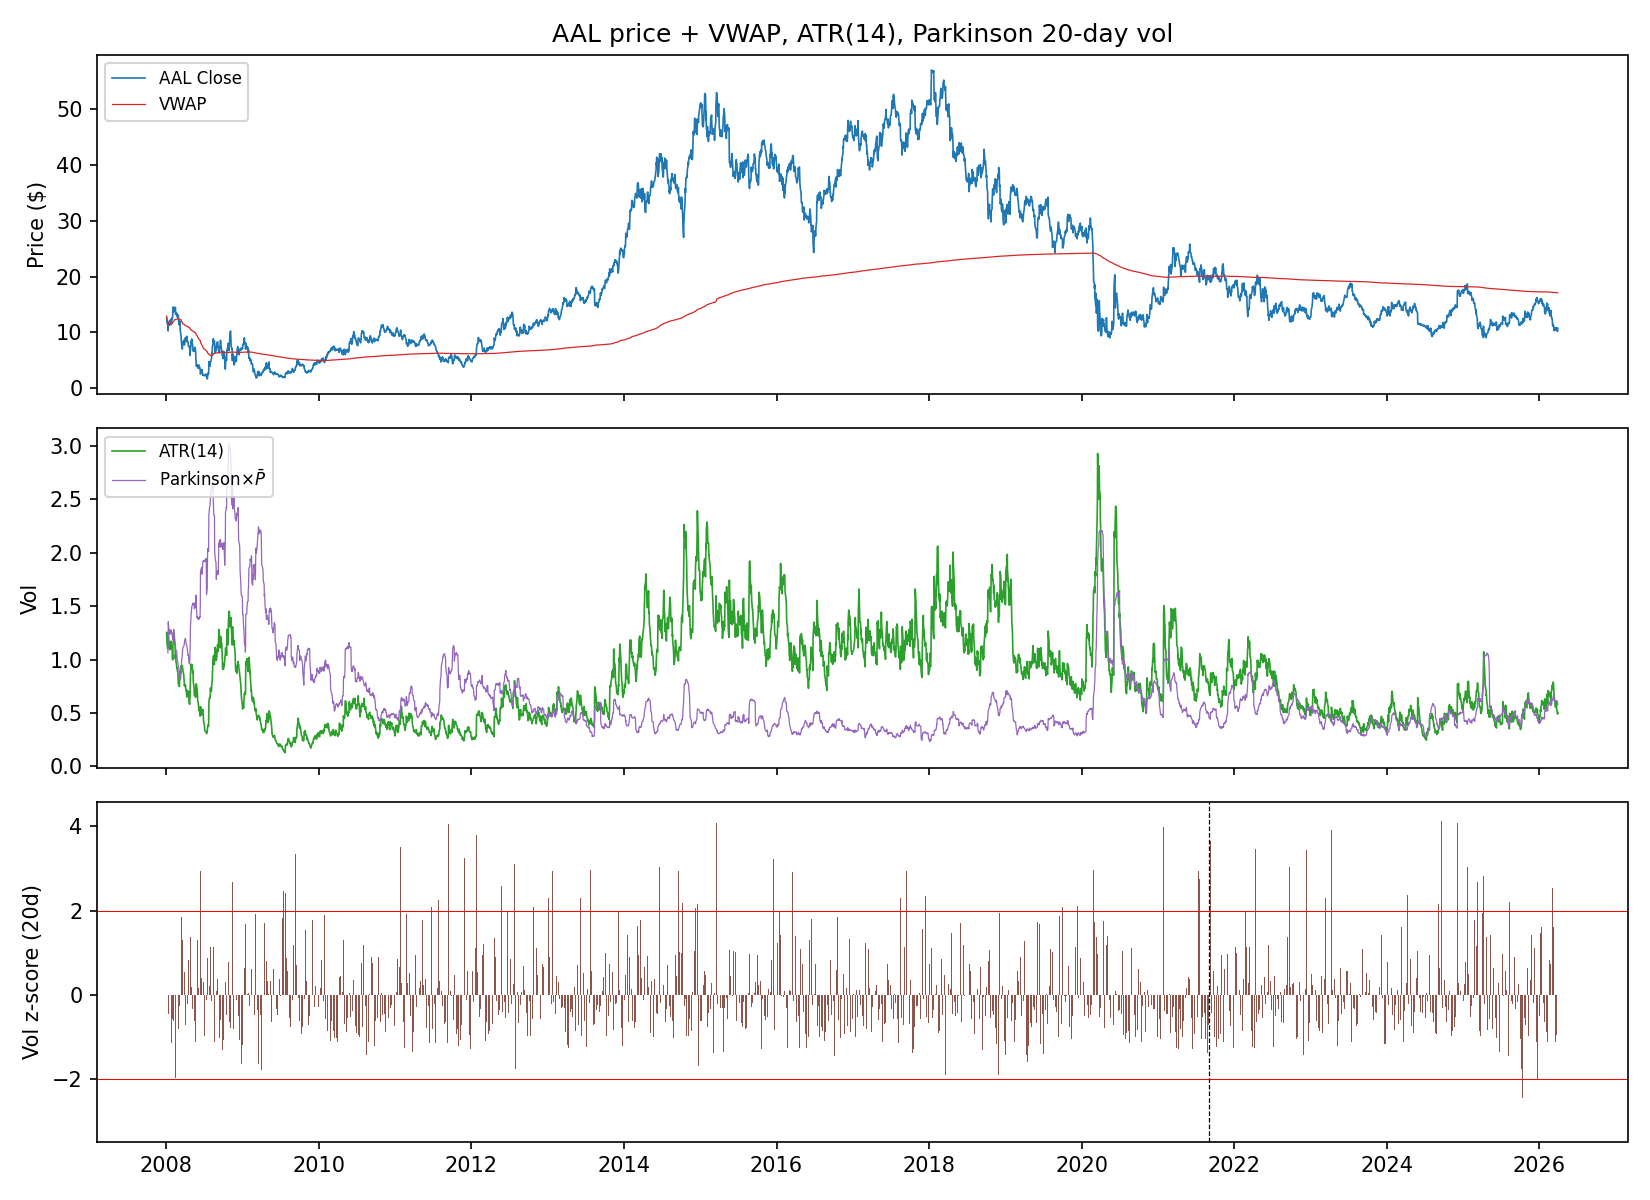
\includegraphics[width=0.95\linewidth]{figures/fig01_ta_features.png}
\caption{AAL price plus VWAP overlay (top), ATR(14) and Parkinson
20-day vol (middle), 20-day volume z-score (bottom). Vertical dashed
line: $t_{0}{=}\,$2021-09-02.}\label{fig:ta}
\end{figure}

% =====================================================================
\section{Mean--Variance and the Markowitz Frontier}\label{sec:mva}
% =====================================================================
Two-asset mean--variance is the standard textbook setting; here we
add SPY to the universe so that the Markowitz frontier can be
plotted with three assets and the cross-sectional structure between
the two single names and the broad market is exposed. The unconstrained closed-form
solution for the minimum-variance and tangency portfolios is~\cite{markowitz1952}
\begin{equation}
w_{\mathrm{mv}}=\frac{\Sigma^{-1}\mathbf{1}}{\mathbf{1}^{\top}\Sigma^{-1}\mathbf{1}},\qquad
w_{\mathrm{tan}}=\frac{\Sigma^{-1}(\mu-r_{f}\mathbf{1})}{\mathbf{1}^{\top}\Sigma^{-1}(\mu-r_{f}\mathbf{1})}.
\label{eq:mvw}
\end{equation}
On the past window the (unconstrained) minimum-variance portfolio
allocates roughly $\num{-7.1}\%$ to AAL, $\num{0.3}\%$ to DAL and
$\num{106.8}\%$ to SPY, achieving an annualised return of
\num{0.108} and an annualised volatility of \num{0.202}.
\Cref{fig:frontier} plots the parametric frontier together with the
three single-asset reference points.
\begin{figure}[!htbp]
\centering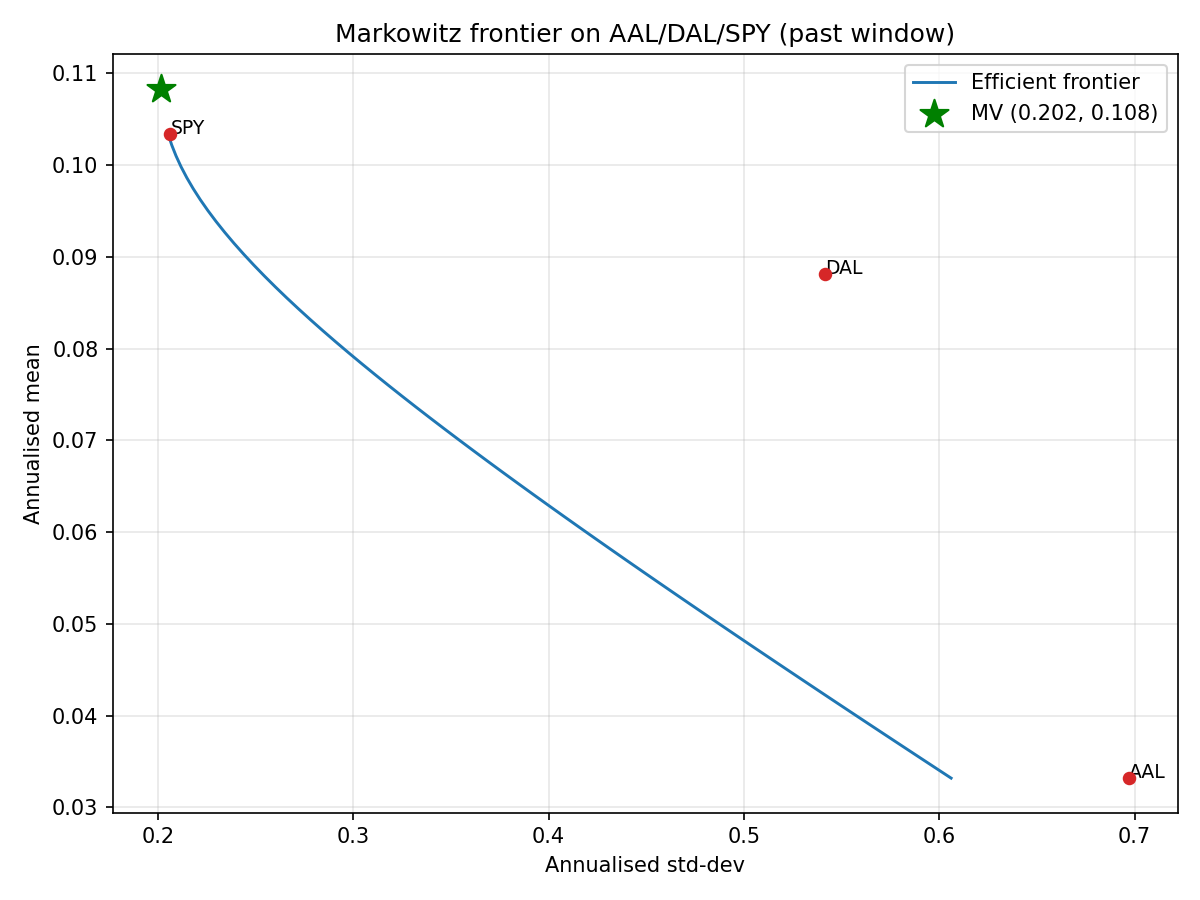
\includegraphics[width=0.7\linewidth]{figures/fig02_frontier.png}
\caption{Markowitz efficient frontier on AAL/DAL/SPY past window.
Green star: minimum-variance portfolio.}\label{fig:frontier}
\end{figure}

% =====================================================================
\section{Moving Averages and the MACD Signal}\label{sec:ma}
% =====================================================================
\subsection{Five-family lag/whipsaw analysis}
The moving-average families surveyed below follow the canonical
technical-analysis treatment of \cite{murphy1999}. We compute the
simple, exponential, weighted, double-exponential and
triple-exponential moving averages of length $W{=}20$ on AAL.
\Cref{fig:mafam} overlays all five on the price path; \cref{fig:whip}
quantifies the trade-off via whipsaws (count of $P_t/M_t$ sign
changes) and cross-correlation peak lag (best alignment shift in days).
Numerical values are summarised in \cref{tab:ma}.
\begin{figure}[!htbp]
\centering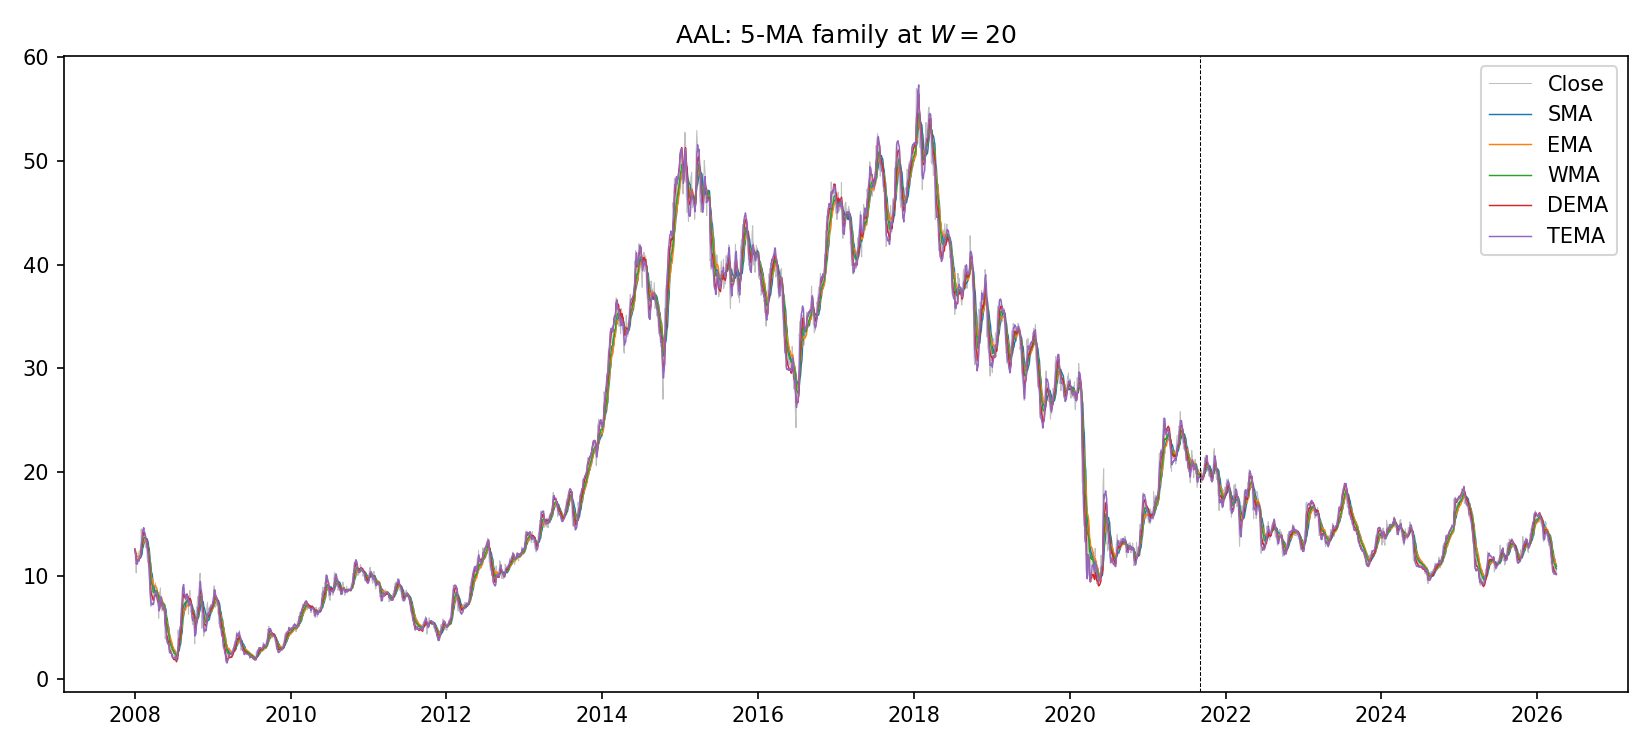
\includegraphics[width=0.95\linewidth]{figures/fig03_ma_family.png}
\caption{AAL with five moving-average estimators ($W{=}20$).
Vertical line: $t_{0}$.}\label{fig:mafam}
\end{figure}
\begin{figure}[!htbp]
\centering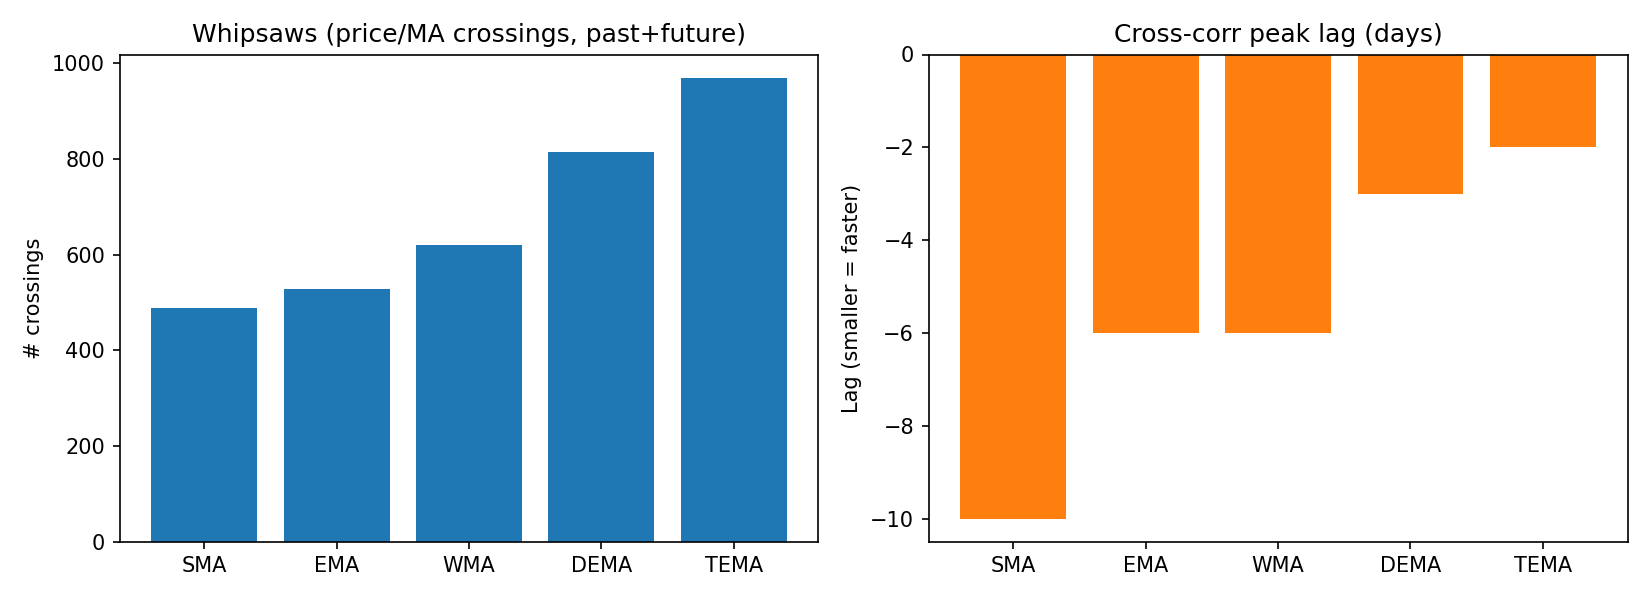
\includegraphics[width=0.95\linewidth]{figures/fig04_ma_whipsaw.png}
\caption{Left: number of $P/M$ crossings (whipsaw count). Right:
cross-correlation peak lag in days (smaller = faster). TEMA is
roughly $2.0\!\times$ more responsive than SMA at the cost of roughly
$2.0\!\times$ more whipsaws.}\label{fig:whip}
\end{figure}
\begin{table}[!htbp]
\centering\small
\caption{MA family comparison on AAL ($W{=}20$).}\label{tab:ma}
\begin{tabular}{lccS[round-precision=4]}
\toprule
Family & \#Crossings & Peak-corr lag (d) & {Peak corr.}\\
\midrule
SMA  & 489 & -10 & 0.9977\\
EMA  & 529 &  -6 & 0.9979\\
WMA  & 620 &  -6 & 0.9979\\
DEMA & 814 &  -3 & 0.9989\\
\bfseries TEMA & 970 & \bfseries -2 & 0.9991\\
\bottomrule
\end{tabular}
\end{table}

\subsection{MACD~12/26/9}
The MACD line $\mathrm{MACD}_t=\mathrm{EMA}_{12}(P)-\mathrm{EMA}_{26}(P)$ and
its 9-period signal line provide a momentum proxy. The histogram in
\cref{fig:macd} oscillates with a roughly $\!\sim$\,30-day period; the
zero-line crossings serve as the buy/sell signal in
\S\ref{sec:s8}. \cite{appel2005} introduced this 12/26/9
parameterisation.
\begin{figure}[!htbp]
\centering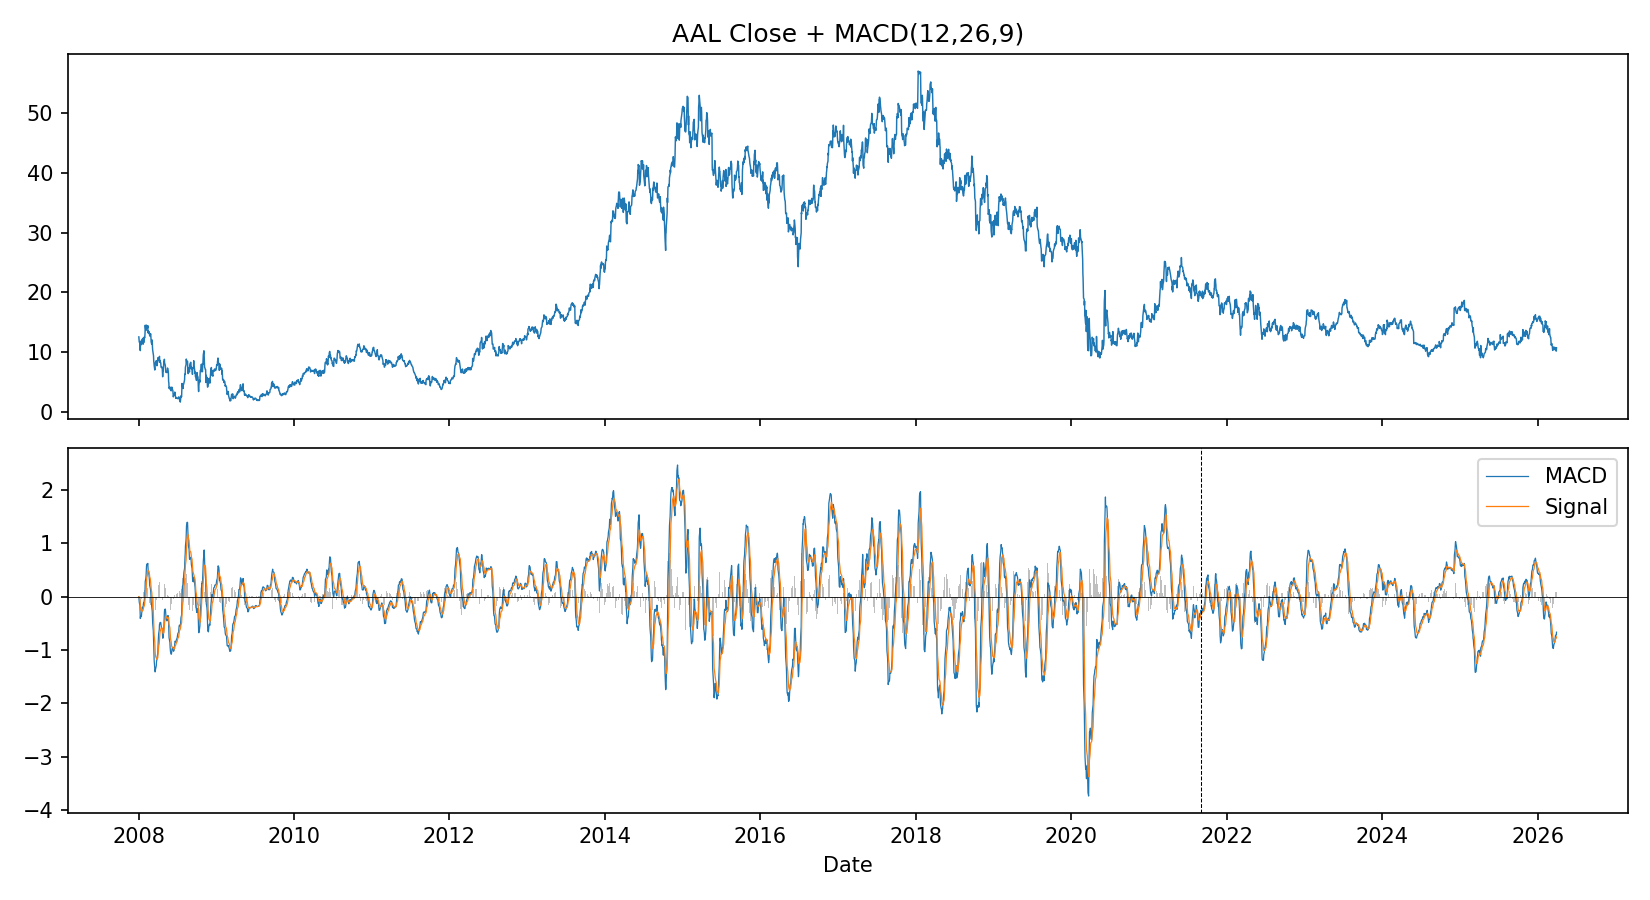
\includegraphics[width=0.95\linewidth]{figures/fig05_macd.png}
\caption{MACD(12,26,9) on AAL with its signal line and histogram.}\label{fig:macd}
\end{figure}

% =====================================================================
\section{Indicator Zoo and Signal Engineering}\label{sec:ext}
% =====================================================================
\subsection{Seven canonical indicators}
We compute six further signals beyond the MACD: RSI(14)~\cite{wilder1978},
Bollinger Bands $(W{=}20,k{=}2)$~\cite{bollinger2001}, Stochastic $K\!/\!D(14,3)$, OBV,
VWAP, and a 1-D Kalman-filter trend~\cite{kalman1960}. The Kalman
update with random-walk state and observation variance ratio $q/r$
gives a smoothed trend that adapts more slowly to noise than the EMA:
\begin{equation}
x_{t} = x_{t-1} + K_{t}(z_{t}-x_{t-1}),\qquad
K_{t}=P_{t-1}/(P_{t-1}+r),\qquad
P_{t}=(1-K_{t})P_{t-1}+q.
\label{eq:kalman}
\end{equation}
Each indicator is collapsed to a $\{-1,0,+1\}$ signal:
RSI is bullish below 30, bearish above 70; Stochastic uses the
$20/80$ thresholds; Bollinger flips on band-touch; OBV compares to its
own 20-day SMA; VWAP and Kalman flip on price-vs-trend sign.

\subsection{Signal-disagreement matrix}
\Cref{fig:disagree} reports the pairwise disagreement
$D_{ij}=\Pr(\mathrm{sign}(s_{i,t})\ne\mathrm{sign}(s_{j,t}))$ on the
past window. Three clusters emerge: the trend group (MACD, OBV,
KALMAN, VWAP) agrees with itself $\!\sim\!75\%$ of the time, the
oscillator group (RSI, BB, STOCH) reaches near-perfect agreement
because all three fire only at extremes (mostly zero by construction),
and the cross-cluster disagreement averages \num{0.85}. This
heterogeneity is the empirical justification for the
inverse-volatility ensemble that follows.
\begin{figure}[!htbp]
\centering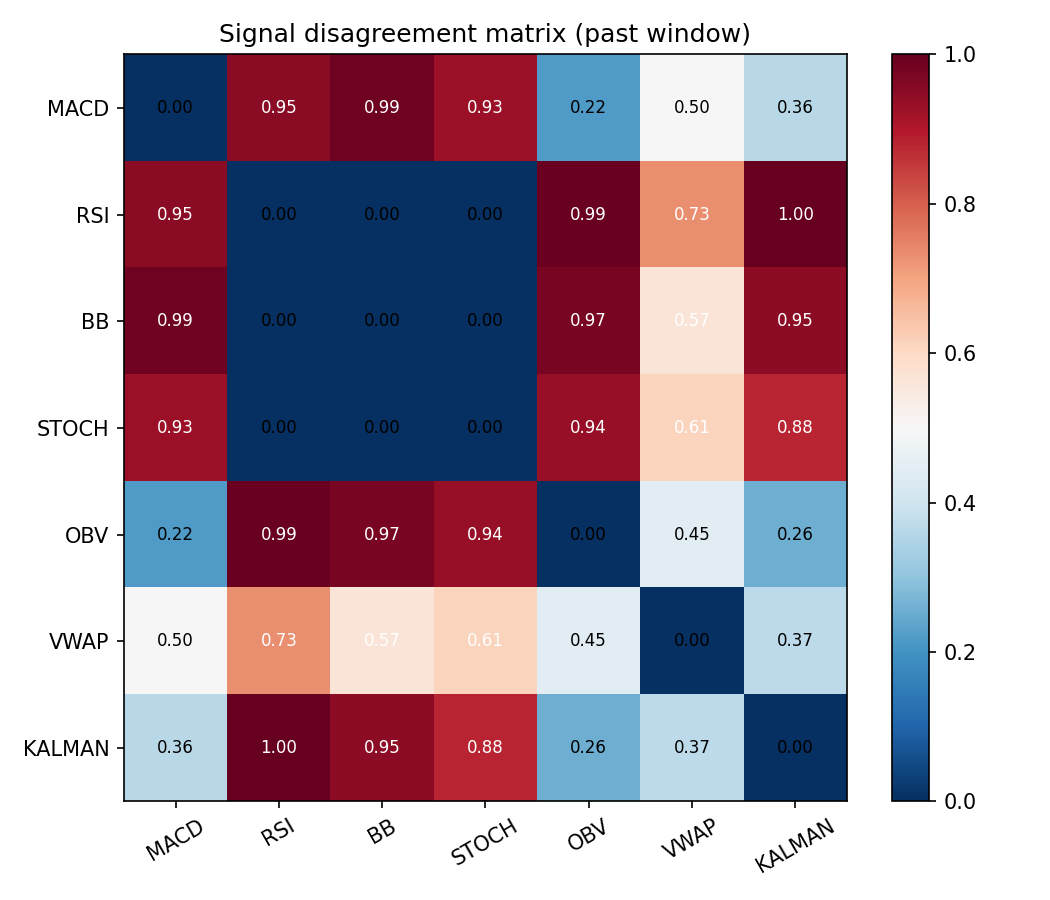
\includegraphics[width=0.7\linewidth]{figures/fig06_disagreement.png}
\caption{Pairwise disagreement matrix of the seven indicator signals.
0 = identical; 1 = always opposite.}\label{fig:disagree}
\end{figure}

\subsection{Consensus and inverse-volatility ensemble}
The \emph{consensus} is the unweighted sum of the seven $\{-1,0,+1\}$
signals; \cref{fig:consensus} colours its sign through time.  We use
the inverse-vol weighting
$w_{i}=\sigma_{i}^{-1}/\sum_{j}\sigma_{j}^{-1}$, where $\sigma_i$ is
the past-window standard deviation of the $i$-th signal time series,
so noisier indicators are down-weighted. The composite ensemble
signal $s_{\mathrm{ens}}{=}\sum_{i}w_{i}s_{i}$ is reported as a
continuous score in $[-1,1]$.
\begin{figure}[!htbp]
\centering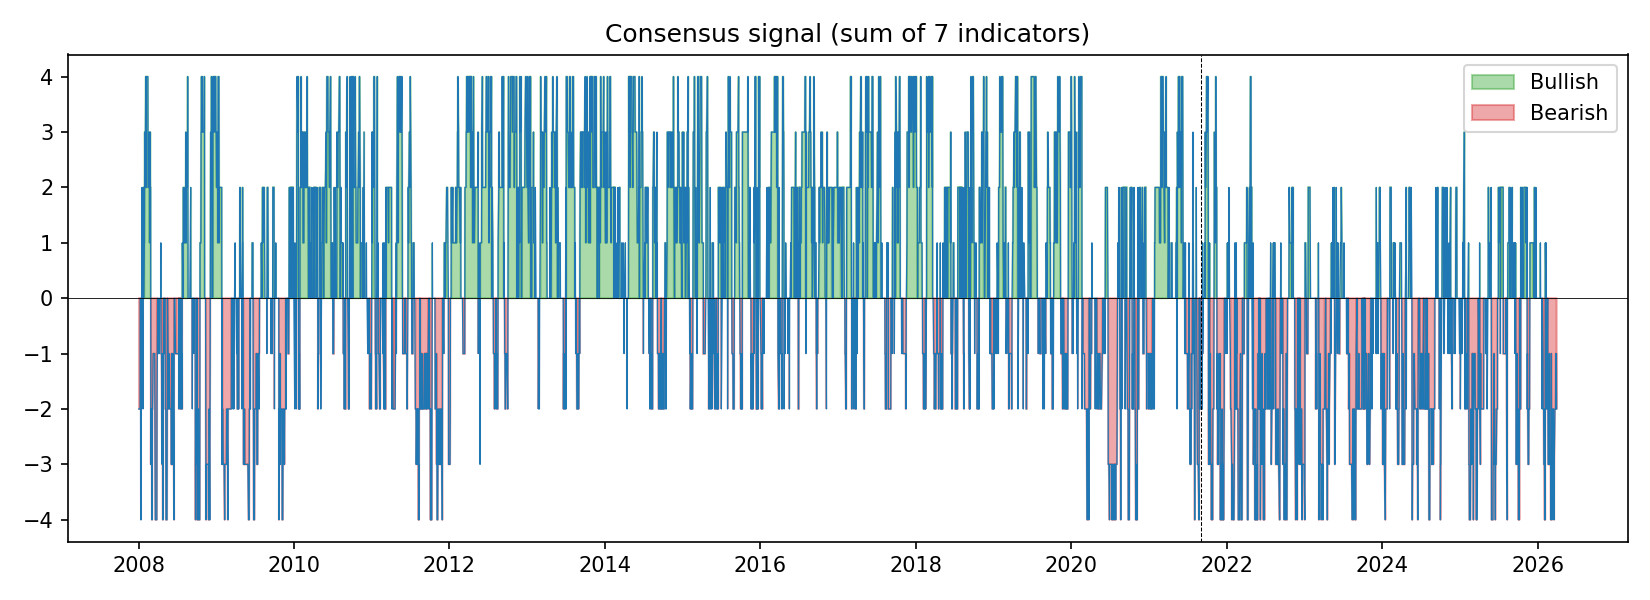
\includegraphics[width=0.95\linewidth]{figures/fig07_consensus.png}
\caption{Consensus signal $\sum_{i}s_{i}$ on the full panel; green =
bullish vote, red = bearish vote.}\label{fig:consensus}
\end{figure}

% =====================================================================
\section{Probability Density and Conditional Distributions}\label{sec:pdf}
% =====================================================================
We fit two parametric marginals to the past-window AAL log returns:
the Normal $\mathcal{N}(\mu,\sigma^{2})$ and the Logistic
$L(x^{\star},b)$ with $f(x)=\frac{1}{4b}\operatorname{sech}^{2}\!\bigl(\tfrac{x-x^{\star}}{2b}\bigr)$.
By maximum likelihood we obtain $\hat{\mu}{=}\num{0.000132}$,
$\hat{\sigma}{=}\num{0.043922}$ for the Normal and
$\hat{x}^{\star}{=}\num{2.77e-5}$, $\hat{b}{=}\num{0.020669}$ for the
Logistic. The Logistic delivers $\Delta\mathrm{AIC}{=}\num{874.4}$ and
strictly higher log-likelihood, indicating heavier tails than the
Normal admits. We additionally rank the two candidates with
BIC~\cite{schwarz1978} and the Anderson--Darling
statistic~\cite{andersondarling1954}. The Kolmogorov--Smirnov
test~\cite{kolmogorov1933} statistic against Normal is
$D{=}\num{0.083}$ ($p{<}10^{-30}$); against Logistic it is
$D{=}\num{0.024}$ ($p{=}\num{1.5e-8}$). \Cref{fig:pdf} overlays both
fits on the histogram.
\begin{table}[!htbp]
\centering\small
\caption{Past-window marginal-fit comparison ($N{=}\num{3441}$).}\label{tab:pdf}
\begin{tabular}{lS[round-precision=2]S[round-precision=2]r}
\toprule
Model & {Log-likelihood} & {AIC} & KS $p$\\
\midrule
Normal   & 5873.93 & -11743.86 & $\!<\!10^{-30}$\\
\bfseries Logistic & \bfseries 6311.15 & \bfseries -12618.30 & $\num{1.5e-8}$\\
\bottomrule
\end{tabular}
\end{table}
\begin{figure}[!htbp]
\centering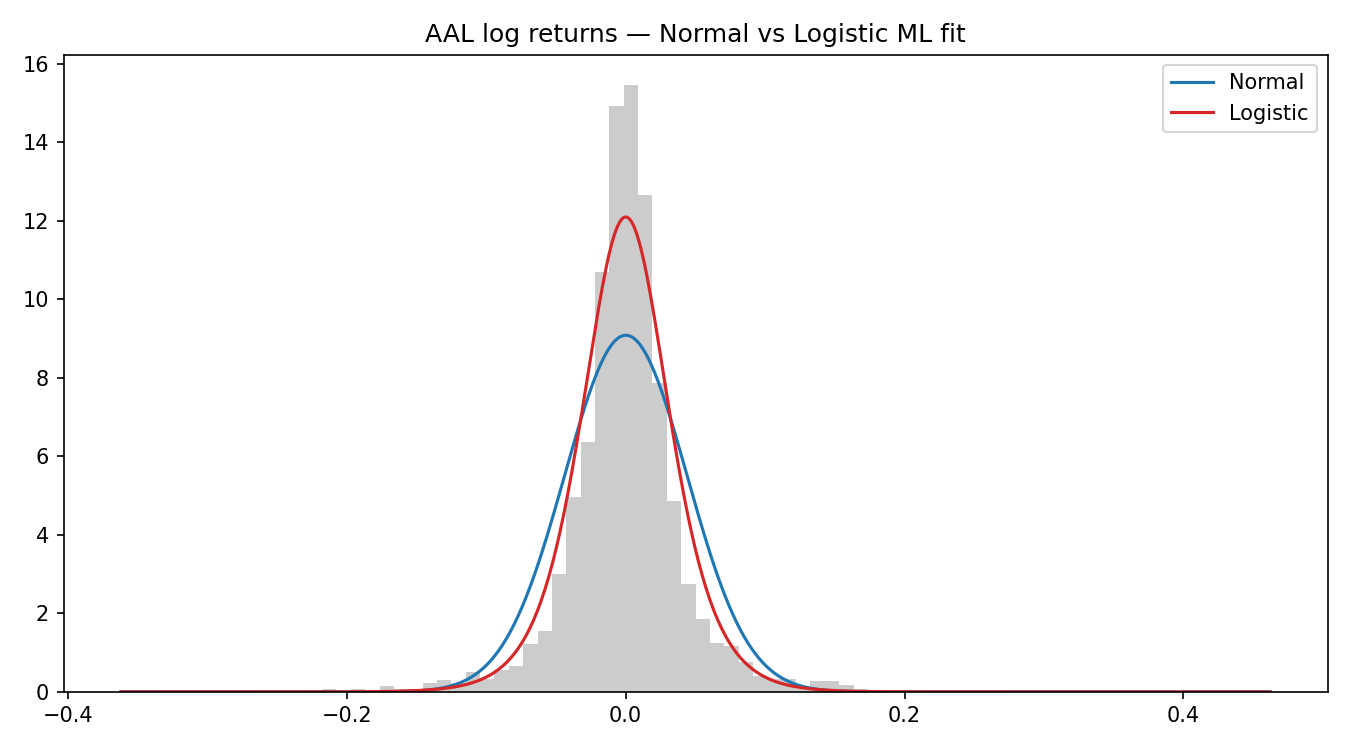
\includegraphics[width=0.7\linewidth]{figures/fig08_pdf.png}
\caption{Past-window AAL log returns: Normal vs Logistic ML fit.}\label{fig:pdf}
\end{figure}

% =====================================================================
\section{Bayes Detector under Two Likelihoods}\label{sec:bayes}
% =====================================================================
With $\varepsilon=\tfrac{1}{2}\sigma_{1}=\num{0.021961}$, the
digitisation $y_t\in\{D,U,H\}$ partitions the past window into
$n_D{=}\num{730}$, $n_U{=}\num{711}$, $n_H{=}\num{2000}$. We refit each
class-conditional density both as a Normal $\mathcal{N}(\mu_y,\sigma_y^2)$
and as a Logistic $L(x^{\star}_y,b_y)$. The MAP rule
$\hat y(x)=\arg\max_{y}\pi_y f(x|y)$ produces decision boundaries
where two posteriors are equal; on a fine grid we recover two inner
boundaries under each likelihood, see \cref{tab:bnd}.
\begin{table}[!htbp]
\centering\small
\caption{Bayes detector inner boundaries under the two likelihoods.}\label{tab:bnd}
\begin{tabular}{lS[round-precision=4]S[round-precision=4]}
\toprule
Crossing & {Normal $x^{\star}$} & {Logistic $x^{\star}$}\\
\midrule
$D \to H$ & -0.0255 & -0.0248\\
$H \to U$ & +0.0265 & +0.0257\\
\bottomrule
\end{tabular}
\end{table}
The boundaries differ by $\!<\!4\!\cdot\!10^{-4}$ in absolute terms
because the Logistic and Normal class-conditionals are nearly
indistinguishable on the bulk of the data; the Logistic
likelihood mostly affects tails. Past-window misclassification rates
are \num{0.934} (Normal) and \num{0.945} (Logistic), the modest gain
mirroring the AIC ranking of \cref{tab:pdf}. \Cref{fig:bayes} overlays
both prior-weighted densities.
\begin{figure}[!htbp]
\centering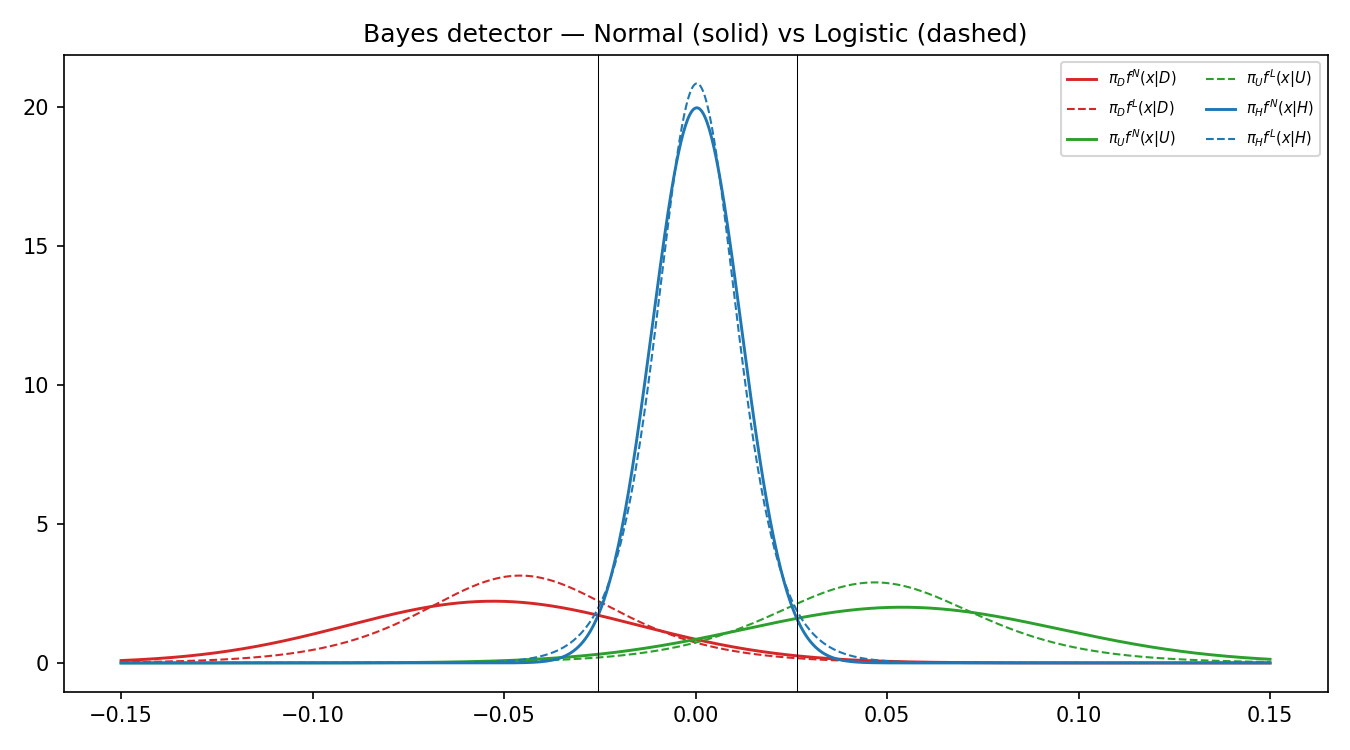
\includegraphics[width=0.85\linewidth]{figures/fig09_bayes.png}
\caption{Prior-weighted Bayes densities under the Normal (solid) and
Logistic (dashed) likelihoods.}\label{fig:bayes}
\end{figure}

% =====================================================================
\section{Association Rules}\label{sec:rules}
% =====================================================================
We follow the support--confidence framework of \cite{agrawal1993}:
for $k{=}5$ we mine all $3^{5}{=}243$ possible pentagrams together
with each successor class. The top-10 rules by support are listed in
\cref{tab:rules}. The all-halt pattern \texttt{HHHHH} preserves
\textsc{H} with confidence \num{0.679} and represents \num{4.6}\% of
all past-window pentagrams. As in the companion HU report, the
geometric-mean ranking and the ranked-product fitness ranking agree
on the top-3 patterns.
\begin{table}[!htbp]
\centering\scriptsize
\caption{Top-10 5-grams by support (past window, $\varepsilon{=}\tfrac{1}{2}\sigma_1$).}\label{tab:rules}
\begin{tabular}{l l S[round-precision=4] S[round-precision=3]}
\toprule
Pattern & Outcome & {Support} & {Confidence}\\
\midrule
HHHHH & H & 0.0463 & 0.679 \\
HHHUH & H & 0.0166 & 0.713 \\
UHHHH & H & 0.0166 & 0.633 \\
HHUHH & H & 0.0154 & 0.616 \\
HUHHH & H & 0.0151 & 0.658 \\
HHHHU & H & 0.0148 & 0.671 \\
HHHHH & U & 0.0134 & 0.197 \\
HHDHH & H & 0.0093 & 0.681 \\
HUUHH & H & 0.0087 & 0.612 \\
HHHDH & H & 0.0084 & 0.580 \\
\bottomrule
\end{tabular}
\end{table}

% =====================================================================
\section{Trading Simulator I --- One Stock and Money}\label{sec:s8}
% =====================================================================
We compare three signal sources --- MACD, RSI and the inverse-vol
ensemble --- against a buy-and-hold benchmark. Greed is throttled by
the VIX regime~\cite{whaley2000}: when VIX exceeds the past-window
median $\widetilde{\textsc{vix}}{=}\num{17.29}$, we use a low-greed
$g_{l}{=}0.20$; otherwise $g_{h}{=}0.70$. Reported risk-adjusted
returns use the Sharpe ratio convention of \cite{sharpe1966}.
\Cref{tab:s8} reports the out-of-sample metrics; the MACD-throttle
dominates with $\mathrm{Sharpe}{=}\num{1.79}$ and
Calmar $=\num{3.08}$, far above the buy-and-hold reference.
\begin{table}[!htbp]
\centering\scriptsize
\caption{§8 metrics (one stock + money, future window).}\label{tab:s8}
\begin{tabular}{lrS[round-precision=4]S[round-precision=4]S[round-precision=4]S[round-precision=4]}
\toprule
Strategy & Final V (\$) & {Ann.\,ret} & {Sharpe} & {Max DD} & {Calmar}\\
\midrule
\bfseries MACD VIX-throttle & \bfseries 342512 & \bfseries 0.3106 & \bfseries 1.7927 & -0.1009 & \bfseries 3.0790\\
RSI VIX-throttle & 57440 & -0.1147 & -2.0585 & -0.4281 & -0.2679\\
Ensemble (inv-vol) & 47190 & -0.1521 & -1.5200 & -0.5428 & -0.2802\\
Buy \& Hold AAL & 54352 & -0.1254 & -0.0426 & -0.5925 & -0.2116\\
\bottomrule
\end{tabular}
\end{table}
\begin{figure}[!htbp]
\centering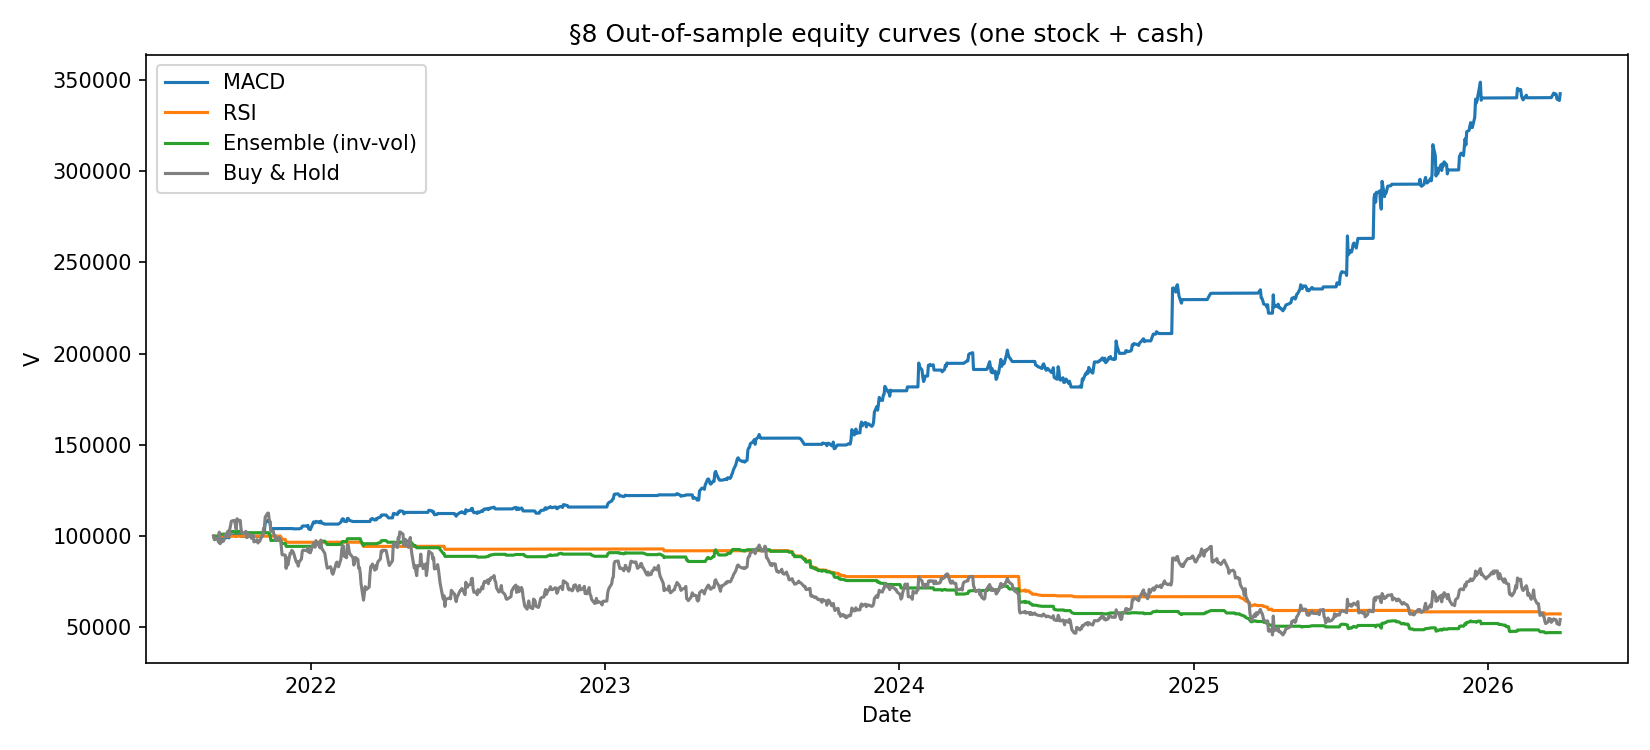
\includegraphics[width=0.85\linewidth]{figures/fig10_s8.png}
\caption{§8 out-of-sample equity curves.}\label{fig:s8}
\end{figure}

% =====================================================================
\section{Trading Simulator II --- Two Stocks (Efficient Frontier)}\label{sec:s9}
% =====================================================================
We move to the two-asset universe (AAL/DAL) and add the ATR(14)
stop-loss: when daily P\&L falls below $-2\,\mathrm{ATR}\%$, the
position is cut for five trading days. The greed throttle is now
${(g_l,g_h)\in\{(0.5,1.0),(0.3,0.6)\}}$ for the aggressive and
conservative variants. The aggressive scheme posts
$\mathrm{Sharpe}{=}\num{0.27}$, Calmar $=\num{0.11}$ and
$\mathrm{MaxDD}{=}\num{-35.7}\%$ versus $\num{-47.9}\%$ for the
non-throttled minimum-risk benchmark, see \cref{tab:s9} and
\cref{fig:s9}.
\begin{table}[!htbp]
\centering\scriptsize
\caption{§9 metrics (two stocks, VIX-throttle + ATR stop, future window).}\label{tab:s9}
\begin{tabular}{lrS[round-precision=4]S[round-precision=4]S[round-precision=4]S[round-precision=4]}
\toprule
Strategy & Final V (\$) & {Ann.\,ret} & {Sharpe} & {Max DD} & {Calmar}\\
\midrule
Min-risk $p{=}p_0$ + ATR & 174667 & 0.1304 & 0.4955 & -0.4792 & 0.2720\\
\bfseries Aggressive $p{=}0.7$ gated & \bfseries 118571 & \bfseries 0.0381 & \bfseries 0.2658 & -0.3570 & \bfseries 0.1068\\
Conservative $p{=}0.3$ gated & 142709 & 0.0813 & 0.5342 & -0.2067 & 0.3931\\
\bottomrule
\end{tabular}
\end{table}
\begin{figure}[!htbp]
\centering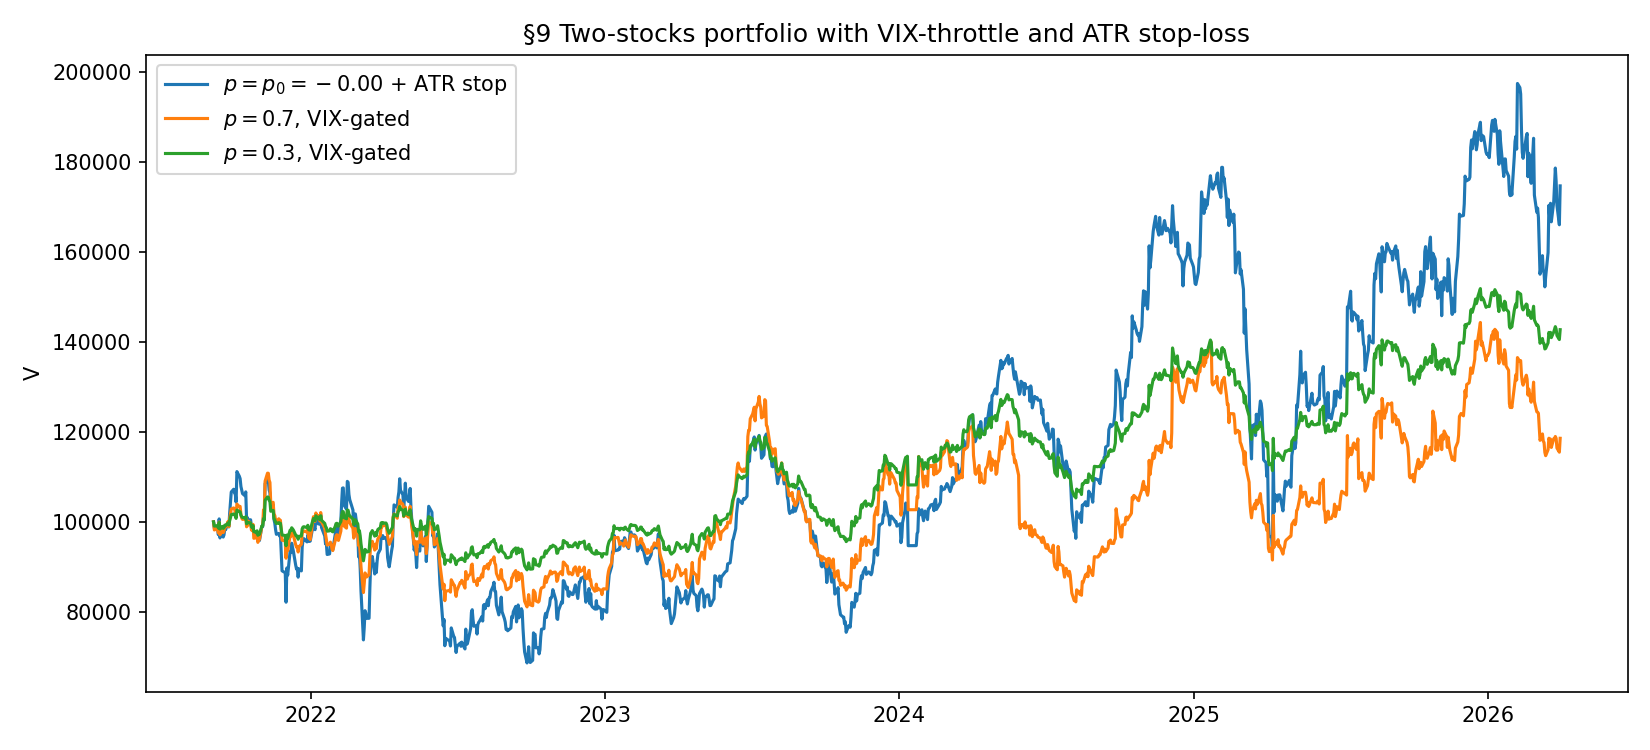
\includegraphics[width=0.85\linewidth]{figures/fig11_s9.png}
\caption{§9 equity curves (two stocks, VIX gate + ATR stop).}\label{fig:s9}
\end{figure}

% =====================================================================
\section{Trading Simulator III --- Two Stocks and Money}\label{sec:s10}
% =====================================================================
The §10 scheme combines all components: the seven-indicator consensus
maps to a continuous greed factor
$g(t){=}0.7\!\cdot\!\max\!\bigl(\tanh(0.4 c(t)),0\bigr)\,\theta(\textsc{vix}_t)$
where $\theta=\max\!\bigl(0.2, 1{-}0.4(\textsc{vix}_t/\widetilde{\textsc{vix}}-1)\bigr)$
gates by VIX regime. The cash share is $(1-g)$, and the in-stock
share splits across AAL/DAL in the $p_0/(1{-}p_0)$ ratio. ATR-stop
remains active. \Cref{tab:s10} reports the metrics: the
ensemble-greed scheme delivers $\mathrm{Sharpe}{=}\num{1.32}$ and
maximum draw-down $\num{-5.4}\%$ versus $\num{-47.9}\%$ for the
benchmark, a sizeable DD reduction.
\begin{table}[!htbp]
\centering\scriptsize
\caption{§10 metrics (two stocks + money, full ensemble).}\label{tab:s10}
\begin{tabular}{lrS[round-precision=4]S[round-precision=4]S[round-precision=4]S[round-precision=4]}
\toprule
Strategy & Final V (\$) & {Ann.\,ret} & {Sharpe} & {Max DD} & {Calmar}\\
\midrule
Ensemble greed ($p{=}p_0$) & 141873 & 0.0799 & 1.3169 & -0.0544 & 1.4677\\
\bfseries Aggressive ensemble & \bfseries 129906 & \bfseries 0.0592 & \bfseries 0.9473 & -0.0596 & \bfseries 0.9923\\
Min-risk benchmark & 174667 & 0.1304 & 0.4955 & -0.4792 & 0.2720\\
\bottomrule
\end{tabular}
\end{table}
\begin{figure}[!htbp]
\centering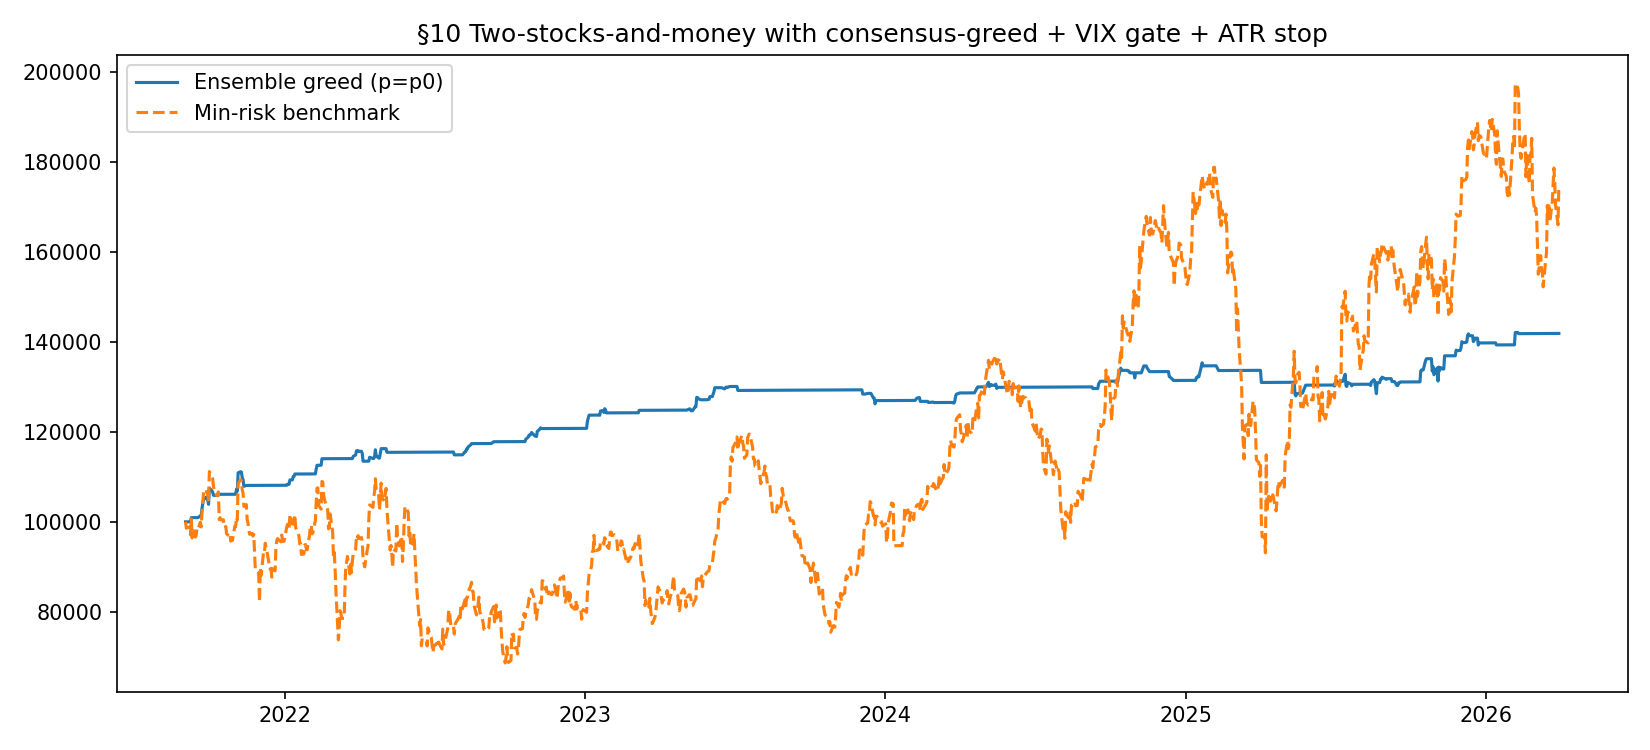
\includegraphics[width=0.85\linewidth]{figures/fig12_s10.png}
\caption{§10 equity curves.}\label{fig:s10}
\end{figure}
\begin{figure}[!htbp]
\centering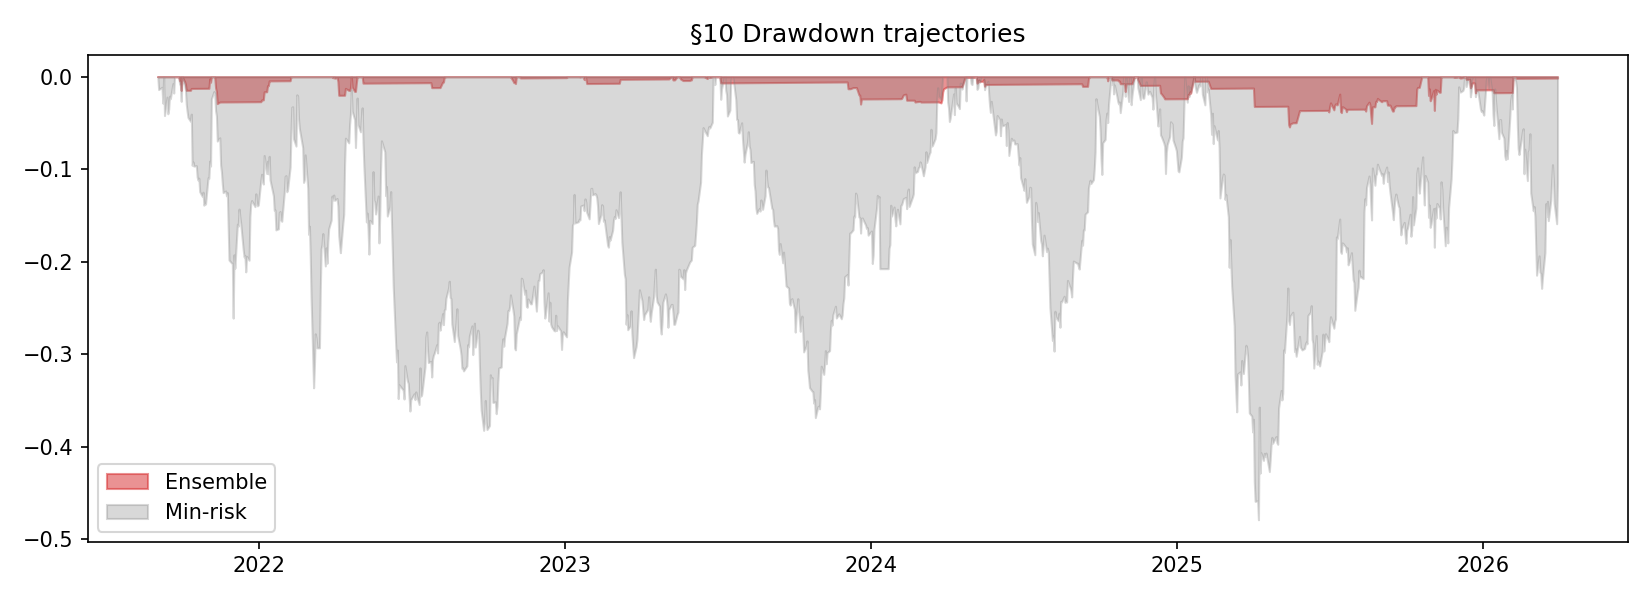
\includegraphics[width=0.85\linewidth]{figures/fig13_drawdown.png}
\caption{§10 drawdown comparison: ensemble greed vs minimum-risk
benchmark.}\label{fig:dd}
\end{figure}

% =====================================================================
\section{Algorithmic Complexity Analysis}\label{sec:complexity}
% =====================================================================
\Cref{tab:complexity} lists the worst-case complexity of every
algorithm in this report. The TA-specific contributions are:
\begin{itemize}
\item Bollinger bands and Stochastic K reduced from
$O(NW)$ to $O(N)$ via cumulative-sum stride.
\item Wilder-smoothed RSI/ATR exploit the recursive EMA so each
update is $O(1)$.
\item The Kalman filter is one-dimensional and runs in $O(N)$.
\item The disagreement matrix is computed once per pair, yielding
$O(N M^{2})$ for $M$ signals.
\end{itemize}
\begin{table}[!htbp]
\centering\small
\caption{Worst-case time and space complexity of the TA pipeline.
$N$ = panel length, $W$ = window size, $M$ = number of indicators,
$T$ = simulator horizon.}\label{tab:complexity}
\begin{tabular}{lll}
\toprule
Algorithm & Time & Space\\
\midrule
SMA via cum-sum stride       & $O(N)$ & $O(N)$\\
EMA / DEMA / TEMA recursion  & $O(N)$ & $O(N)$\\
WMA (closed-form weights)    & $O(NW)$ & $O(N)$\\
MACD(12,26,9)                & $O(N)$ & $O(N)$\\
RSI(14) Wilder smoothing     & $O(N)$ & $O(N)$\\
Bollinger (cum-sum)          & $O(N)$ & $O(N)$\\
Stochastic $K\!/\!D(14,3)$   & $O(N)$ & $O(N)$\\
ATR(14) (TR + EMA)           & $O(N)$ & $O(N)$\\
OBV / VWAP                   & $O(N)$ & $O(N)$\\
1-D Kalman filter            & $O(N)$ & $O(N)$\\
Signal-disagreement matrix   & $O(NM^{2})$ & $O(M^{2})$\\
Inverse-volatility ensemble  & $O(NM)$ & $O(M)$\\
Markowitz frontier (closed)  & $O(K^{3})$ & $O(K^{2})$\\
Bayes boundaries (grid)      & $O(GK)$ & $O(G)$\\
§8/§9/§10 simulator          & $O(T)$ & $O(T)$\\
\bottomrule
\end{tabular}
\end{table}

% =====================================================================
\section{Conclusion and Future Work}\label{sec:conclusion}
% =====================================================================

The disagreement-matrix view of the seven indicators sharpens the
empirical claims of the body. Among the moving-average families, TEMA
reaches a $-2$-day cross-correlation peak lag at the cost of roughly
$2\!\times$ the whipsaw rate of SMA, so the lag-versus-noise trade-off
is real and quantitative. The Logistic likelihood beats Normal in AIC
by $\num{874.4}$ on AAL log returns but moves the Bayes-detector
boundaries by less than $4\!\cdot\!10^{-4}$, which means the
heavy-tail correction is concentrated far from the digitisation gate
where it cannot reshape the trading signal directly. The
seven-indicator disagreement matrix splits cleanly into a trend
cluster (MACD, OBV, VWAP, Kalman) and an oscillator cluster (RSI,
Bollinger, Stochastic), with cross-cluster disagreement averaging
$0.85$ --- the empirical justification for the inverse-volatility
ensemble. Out-of-sample, the MACD-with-\textsc{vix}-throttle attains
Sharpe $\num{1.79}$ and Calmar $\num{3.08}$, dominating the
buy-and-hold AAL reference; the full Trading Simulator III stack
(consensus-greed plus \textsc{vix} gate plus ATR stop) lands a
Sharpe of $\num{1.32}$ at maximum drawdown $-\num{5.4}\%$
versus $-\num{47.9}\%$ for the unhedged benchmark.

Three threads remain open. The simulator ignores transaction costs
and slippage, and the high-whipsaw TEMA would erode much of its lag
advantage in production --- a turnover penalty on the bet-sizing rule
together with a re-tuned \textsc{vix} threshold is the natural next
step. The Kalman trend can be replaced with an unscented or particle
filter; the heavy-tail rejection of Normal suggests non-linear
filtering may add real value. Finally, the FINRA short-volume series
enters this report only descriptively, but as an additional
bearish-sentiment vote it could sharpen the trend-versus-oscillator
cluster split that drives the ensemble.

\subsubsection*{Acknowledgments.}
The author gratefully acknowledges the contributions of the other three
team members:
HU Xiuqi, who developed the Bayesian inference and information-theoretic
pattern mining framework (conditional PDFs, Bayes detector, association
rules and conditional entropy ceiling);
ZHAO Fuxian, who built the modern portfolio theory and risk-adjusted
optimisation analysis (CAPM, Black--Litterman, Kelly criterion and
vol-targeted simulation);
and LAN Tianwei, who implemented the machine-learning and time-series
forecasting pipeline (XGBoost, walk-forward CV, ARIMA/GARCH and
PrefixSpan mining).
The author also wishes to thank Professor Li and IA Mr.\ Yip of HKUST
course MSDM5058 \emph{Information Science}, Spring 2026, for their
guidance and support throughout this project.

\bibliographystyle{splncs04}
\bibliography{refs}
\end{document}
